\documentclass[a4paper]{article}
\usepackage[english]{babel}
\usepackage{graphicx}
\usepackage{listings}
\usepackage{xcolor}
\usepackage{graphicx}

\pagecolor{white}
\definecolor{codegreen}{rgb}{0,0.6,0}
\definecolor{codegray}{rgb}{0.5,0.5,0.5}
\definecolor{codepurple}{rgb}{0.58,0,0.82}
\definecolor{codeorange}{rgb}{0.8,0.5,0.1}
 
\lstdefinestyle{mystyle}{
    commentstyle=\color{codegreen},
    keywordstyle=\color{codeorange},
    numberstyle=\tiny\color{codegray},
    stringstyle=\color{codegreen},
    basicstyle=\ttfamily\footnotesize,
    breakatwhitespace=false,         
    breaklines=true,                 
    captionpos=b,                    
    keepspaces=true,                 
    numbers=left,                    
    numbersep=5pt,                  
    showspaces=false,                
    showstringspaces=false,
    showtabs=false,                  
    tabsize=2
}
 
\lstset{style=mystyle}

\begin{document}

\author{Federico Fregosi \and Mirko Laruina \and Riccardo Mancini \and Gianmarco Petrelli}
\title{Tutorial JPA}
\maketitle
\vspace{3cm}
\tableofcontents

\newpage
This tutorial is provided to explain and highlight the main techniques and advantages developed by JPA (Java Persistence API), a Java API specification for relational data management in applications using Java SE and Java EE.

\section{What is JPA?}
In order to use jpa within our application (we have totally implemented the middleware that manages the db connections via JAVA), it is necessary to introduce a framework that implements this ORM system.

ORM (Object Relational Mapping) is a programming technique that favors the integration of software systems adhering to the object-oriented programming (OOP) paradigm with RDBMS systems. An ORM implementation provides, through an object-oriented interface, all the services related to data persistence, while abstracting the implementation features of the specific RDBMS used. His main goal is object-relational impedance mismatch resolution. JPA is Java standard specification for ORM and we decided to use and analyze the implementation offered by the Hibernate framework.

Hibernate ORM (Hibernate in short) is an object-relational mapping tool for the Java programming language. It provides a framework for mapping an object-oriented domain model to a relational database. Hibernate handles object-relational impedance mismatch problems by replacing direct, persistent database accesses with high-level object handling functions.
Hibernate's primary feature is mapping from Java classes to database tables and mapping from Java data types to SQL data types. Hibernate also provides data query and retrieval facilities. It generates SQL calls and relieves the developer from the manual handling and object conversion of the result set.

\section{Entity}
Entities represent persistent data stored in a relational database automatically using container-managed persistence.They are persistent because their data is stored persistently in some form of data storage system, such as a database. In general, an entity represents a table stored in a database.

Here an example of how to create an entity:
\lstinputlisting[language=Java]{code1.java}

This class has the task of managing the “messages” entity within the DBMS.

\textbf{@Id}: Marks the field as the key of the entity.

\textbf{@GeneratedValue(strategy=GenerationType.IDENTITY)}: Set the field to follow DB inner configuration.
\textbf{@GeneratedValue} in general it specifies the generation strategy and refers to the name of the generator.

\textbf{@Transient}: The fields marked as transient are not evaluated for persistence, just like the transient
keyword for serialization. In this example we have two fields which won’t be  written on DB.

\textbf{@Column}: This annotation mentions the details of a column, if missing, the name of the field will be considered the name of the column in the table.
You can use \textbf{@basic} for not mismatching fields. A basic type maps directly to a column in the database. These include Java primitives and their wrapper classes, String, java.math.BigInteger and java.math.BigDecimal, various available date-time classes, enums, and any other type that implements java.io.Serializable.

\section{Persitence.xml}
In JPA, the persistence.xml file is the central piece of configuration. That makes it one of the most important files of your persistence layer. It defines one or more persistence units, and here you can configure things like the name of each persistence unit, which managed persistence classes are part of a persistence unit, several provider-specific configuration parameters, and much more.

Here our persistence.xml file is shown:
\lstinputlisting[language=XML]{code2.xml}

In the sixth row we define the name of our persistence-unit without defining a dependency to a specific JPA implementation. After that, a list of proprieties are defined in order to provide the database connection:

\begin{itemize}
\item\textbf{javax.persistence.jdbc.url} – The connection URL of your database
\item\textbf{javax.persistence.jdbc.user} – The user name to login to your database
\item\textbf{javax.persistence.jdbc.password} – The password to login to your database
\item\textbf{javax.persistence.jdbc.driver} – The fully qualified class name of your JDBC driver
\end{itemize}

After that, hibernate is configured as persistence provider by specifying MySql as dialect of the persistence engine with the \textbf{hibernate.dialect} propriety. Finally, some other proprieties are defined in order to enable the logging of all the generated SQL statements to the console (\textbf{hibernate.show\_sql}) and format the generated SQL statement to make it more readable, but takes up more screen space (\textbf{hibernate.format\_sql}).

\section{Relations}
After the declaration of the entity, in our Java classes we can find the declaration of the relationship between entities. Here the entity classes are treated as relational tables (concept of JPA), therefore the relationships between Entity classes are as follows:

\begin{itemize}
\item{@OneToOne Relation}
\item{@OneToMany Relation}
\item{@ManyToOne Relation}
\item{@ManyToMany Relation}
\end{itemize}
For all those types of relationship it's necessary that the two entities involved belong to the same package.

\subsection{@OneToOne Relations}
In One-To-One relationship, one item can belong to only one other item. It means each row of one entity is referred to one and only one row of another entity.
One way to make this association is using a shared primary key i.e. marking the primary key column of the address table as the foreign key to the users table. This avoid us to create a new column, necessary if we wanted to manage the relation between a foreign key.

Here an example of a one-to-one relation between a table 'users' and a table 'address':
\lstinputlisting[language=Java, firstline=1, lastline=12]{code0.java}
\lstinputlisting[language=Java, firstline=14, lastline=25]{code0.java}

The two elements that we want to correlate are marked by the \textbf{@OneToOne} annotation while @MapsId tells Hibernate to use the id column of address as both primary key and foreign key. Moreover the \textbf{mappedBy} attribute is put in the User class since the foreign key is now present in the address table.

\subsection{@OneToMany Relations}
In this relationship each row of one entity is referenced to many child records in other entity. The important thing is that child records cannot have multiple parents. In a one-to-many relationship between Table A and Table B, each row in Table A is linked to 0, 1 or many rows in Table B.

Sometimes this type of relation is bidirectional: a one-to-many relation from an entity A to an entity B, makes it necessary to have a many-to-one relation form the entity B to the entity A.

Here an example of a one-to-many relation from our project:
\lstinputlisting[language=Java]{code3.java}

In this example every element 'chat' of the entity Chats is associated, through the \textbf{mappedBy} propriety, with 0, 1 or many objects of type Message, the other entity involved. In order to do this, an array of element Message is created. With the \textbf{cascade = \{ CascadeType.ALL \}} propriety, when we perform some action on the target entity, the same action will be applied to the associated entity.

\subsection{@ManyToOne Relation}
The many-to-one mapping represents a single-valued association where a collection of entities can be associated with the similar entity. Hence, in relational database any more than one row of an entity can refer to the similar rows of another entity.

Here an example of a many-to-one relation from our project:
\lstinputlisting[language=Java]{code4.java}

The \textbf{@JoinColumn} parameter specifies the database table column that stores the foreign key for the related entity, and then an object with type or the related entity is created.

Note that this relation is the inverse of the one-to-many relation showed in the previous example. This because, as i said before, this can be a bidirectional relation. 

\subsection{@ManyToMany Relation}
The many-to-many mapping represents a collection-valued association where any number of entities can be associated with a collection of other entities. In relational database any number of rows of one entity can be referred to any number of rows of another entity.

For example, in our project, a user can have multiple chat and a chat can be composed of many members.

\begin{figure}[h]
\centering
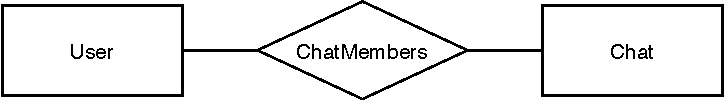
\includegraphics[width=0.75\textwidth]{dia1.pdf}
\end{figure}

As we know, in RDBMSes we can create relationships with foreign keys. Since both sides should be able to reference the other, we need to create a separate table to hold the foreign keys:

\begin{figure}[h]
\centering
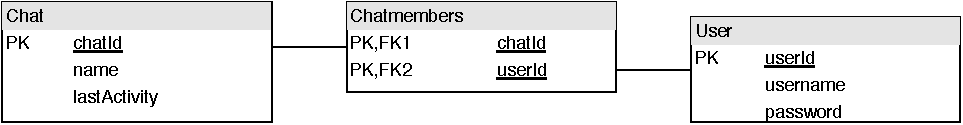
\includegraphics[width=0.90\textwidth]{dia2.pdf}
\end{figure}

Such a table is called a join table. In the join table, the combination of the two foreign keys will be its composite primary key.

Here an example of a many-to-many relation from our project:
\lstinputlisting[language=Java]{code5.java}

The \textbf{@JoinTable} parameter specifies the name of the table to use as a jpa join table from many-to-many between Chats and Users using name = "Chatmembers". This is because it is not possible to determine the ownership of a many to many jpa mappings because the database tables do not contain foreign keys to refer to other tables. \textbf{@JoinColumn} specifies the name of the column that will refer to the entity to be considered as the owner of the association while \textbf{@inverseJoinColumn} specifies the name of the reverse side of the relationship. In our case we chose Chat as the owner so that @JoinColumn refers to the 'chatId' column in the join table Chatmembers and @InverseJoinColumn refers to userId which is the inverse side of the mapping. As happen is the one-to-many relation, an array of element User is created.

Note that \textbf{@ManyToMany} annotation in the User entity shows an inverse relationship, so use \textbf{mappedBy = members} to refer to the field in the Chat entity:
\lstinputlisting[language=Java]{code6.java}

Since a many-to-many relationship doesn't have an owner side in the database, we could configure the join table in the User class and reference it from the Chat class, obtaining the same result.

\section{Persitence operations}
With JPA, it's possible to perform various operations on an entity such as:

\begin{itemize}
\item{Inserting an Entity}
\item{Finding an Entity}
\item{Updating an Entity}
\item{Deleting an Entity}
\end{itemize}

In order to do those operation, first of all it's necessary to create an entity manager factory object connected to the database with the \textbf{createEntityManagerFactory()} method. The role of this method is to create and return an EntityManagerFactory for the named persistence unit. Thus, this method contains the name of persistence unit passed in the Persistence.xml file.
\lstinputlisting[language=Java]{code7.java}

After that, when we want to operate, we first need to obtain an entity manager from factory with the \textbf{createEntityManager()} method, and, if we want to apply some changes to the data stored in the database, to initialize it with the \textbf{getTransaction().begin()} method. Finally, if we began a transaction, the operation has to be closed (\textbf{getTransaction().commit()}), but in any case it's necessary to release the factory resources (\textbf{close()}).
All those passages are present in the following examples.
Note that all those operations are influenced by "lazy loading": it means that an entity will be loaded only when you actually accesses the entity for the first time. This can help improve the performance significantly since often you won't need the children and so they will not be loaded.
All the operations are illustrated below.

\subsection{Insert}
In JPA, we can easily insert data into database through entities. The EntityManager provides \textbf{persist()} method to insert records.

Here an example of how we inserted users into the database:
\lstinputlisting[language=Java]{code8.java}

After the execution of the program, the student table is generated under MySQL workbench.This table contains the user details.

In case data we want to add belong to a one-to-many or many-to-many relation, a little more attention is required in order to maintain the relation: the \textbf{getReference} method is used to retrieve information from the related tables. getReference is similar to the \textbf{find} method but unlike it, the getReference only returns an entity Proxy which only has the identifier set. If you access the Proxy, the associated SQL statement will be triggered as long as the EntityManager is still open. However, in this case, we don’t need to access the entity Proxy. We only want to propagate the foreign key to the underlying table record so loading a Proxy is sufficient for this use case. So it is a realization with help of "lazy loading".

Here an example of this operation:
\lstinputlisting[language=Java, firstline=5, lastline=12]{code12.java}

 \textbf{getReference} is used also in the management of insert that imply a many-to-one relation. In this case the procedure is easy and similar to a simply entity creation

Here an example of this operation:
\lstinputlisting[language=Java, firstline=54, lastline=60]{code12.java}

\subsection{Find}
To find an entity, EntityManger interface provides \textbf{find()} method that searches an element on the basis of primary key.

Here an example of how we find users into the database:
\lstinputlisting[language=Java]{code9.java}

\subsection{Update}
JPA allows us to change the records in database by updating an entity.

Here an example of how we update data into the database:
\lstinputlisting[language=Java]{code10.java}

\textbf{Merge} creates a new instance of your entity, copies the state from the supplied entity, and makes the new copy managed. The instance you pass in will not be managed (any changes you make will not be part of the transaction unless you call merge again).

\subsection{Delete}
To delete a record from database, EntityManager interface provides remove() method. The remove() method uses primary key to delete the particular record.

Here an example of how we delete data into the database:
\lstinputlisting[language=Java]{code11.java}

In the same way we did for the insert, little precautions need to be taken to manage delete in case of one-to-many or many-to-many relation with the usage of the \textbf{getReference} method.

Here an example of this operation:
\lstinputlisting[language=Java, firstline=29, lastline=36]{code12.java}

\end{document}